
\begin{frame}{Appendix --- Compositional Neutrality (Mayoral): Renewal and the Entrant Typology}
\hypertarget{src:entrant}{}
\small
\textbf{Mayoral race.} Vote-weighted share going to \textbf{first-time candidates}, \textbf{serial challengers}, and \textbf{cross-cycle returners} --- a finer cut of the renewal-vs-entrenchment question than the binary new/incumbent split. Tests whether judicialization changes the \emph{kind} of entrant the votes flow to. Dots are the 2SLS effect of a one-SD judicialization shock, with 90\% (thick) and weak-IV tF (thin) intervals.
\smallskip
\begin{center}
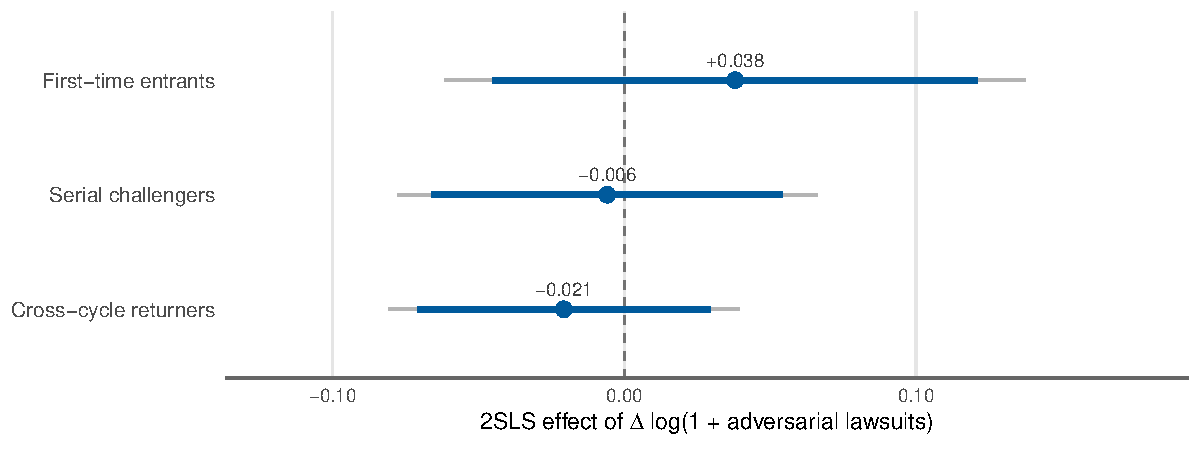
\includegraphics[width=\linewidth,height=0.50\textheight,keepaspectratio]{../figures/entrant_coefplot.pdf}
\end{center}
\smallskip
\footnotesize \textbf{Precise null:} first-timer, serial-challenger, and returner vote shares are all unmoved --- every interval crosses zero. No evidence that litigation shifts the vote toward or away from any class of challenger on net.\hfill\hyperlink{app:entrant}{\beamergotobutton{Full table}}
\end{frame}
